To further demonstrate how the eigenspace overlap metric can be used to better understand the performance of compressed embeddings, in this section we show that we can upper bound the eigenspace overlap for uniformly quantized embeddings.
Given the above theoretical and empirical connections between eigenspace overlap and generalization performance, these bounds help explain why the uniformly quantized embeddings perform so well.
To prove these bounds, we leverage the classic Davis-Kahan $\sin(\Theta)$ theorem from matrix perturbation analysis \citep{sintheta70}.
Because we know exactly what the noise structure of the uniform quantization method is, we can use this knowledge to bound how much the eigenspace of the compressed embeddings can differ from the uncompressed embeddings.

We now present the result (see Appendix~\ref{app:theory} for proof):
\begin{theorem}
	Let $X \in \RR^{n\times d}$ be a bounded embedding matrix with $X_{ij} \in [-\frac{1}{\sqrt{d}},\frac{1}{\sqrt{d}}]$ with smallest singular value $\sigma_{\min} = a \sqrt{n/d}$, for $a \in [0,1]$.\footnote{The maximum possible value of $\sigma_{\min}$ is $\sqrt{n/d}$, which occurs when $\|X\|_F^2 = n$ and $\sigma_{\min} = \sigma_{\max}$.}
	Then the eigenspace overlap of the corresponding $b$-bit uniformly quantized embedding matrix can be lower bounded as follows:
	\begin{eqnarray*}
		%\eigover(X,\tX) &\geq& 1 - \frac{16n}{d(2^b-1)^2} \Bigg( \frac{\sigma_{\max} + \frac{\sqrt{n}}{2^b-1} }{\sigma_{\min}^2} \Bigg)^2
		\expect{}{1-\eigover(X,\tX)} &\leq& \frac{20 \delta_b^2}{a^4}
	\end{eqnarray*}
\label{thm1}
\end{theorem}

This theorem directly results in the following corollary:
%\begin{corollary}
%If $b \geq \log_2\bigg(\frac{8n}{\sigma_{\min}^2 \sqrt{\rho \, d} }} + 1\bigg)$, then the $b$-bit uniformly quantized embedding matrix $\tX$ satisfies $\eigover(X,\tX) \geq 1-\rho$.
%\end{corollary}
\begin{corollary}
	$$\expect{}{1-\eigover(X,\tX)} \leq \eps \;\;\text{if}\;\; b \geq \log_2\bigg(\frac{\sqrt{20}}{a^2\sqrt{\eps}}+1\bigg).$$
\end{corollary}
The corollary shows that one can attain an expected eigenspace overlap arbitrarily close to $1$ if a sufficient number of bits $b$ are used.

\paragraph{Empirical Validation of Theory}
We now validate the above theory by showing the impact of the precision ($b$), the scalar ($a$), the vocabulary size ($n$), and the embedding dimension ($d$) on the eigenspace overlap $\eigover(X,\tX)$ of uniformly quantized embeddings matrices.
As predicted by the theory, we will show in Figure~\ref{fig:micro_eigoverlap} that $1-\eigover(X,\tX)$ drops as $b$ and $a$ are increased, and is relatively unaffected by changes in $n$ and $d$.

We now describe our experimental protocol for studying the impact of each of these parameters on the eigenspace overlap:
\begin{itemize}
	\item \textbf{Precision ($b$), Figure~\ref{fig:micro_eigoverlap}(a)}: We randomly generate a $10^4 \times 10$ matrix, with entries drawn uniformly from $[-\frac{1}{\sqrt{10}},\frac{1}{\sqrt{10}}]$. 
	We uniformly quantize this matrix with precisions $b \in \{1,2,4,8,16\}$, and compute the eigenspace overlap between the quantized matrix and the original matrix.
	As one can see, $1-\eigover(X,\tX)$ drops rapidly as the precision is increased.
	\item \textbf{Scalar ($a$), Figure~\ref{fig:micro_eigoverlap}(b)}: We randomly generate a $10^4 \times 10$ matrix, with entries drawn uniformly from $[-\frac{1}{\sqrt{10}},\frac{1}{\sqrt{10}}]$.
	We then multiply this matrix on the right by diagonal matrices with diagonal entries spaced logarithmically between 1 and $\{1, 0.1,.01,.001,.0001\}$, thus generating matrices with increasingly small values of the scalar $a$.
	We uniformly quantize each of these matrices with precisions $b \in \{1,2,4\}$, and compute the eigenspace overlap between the quantized matrices and the original matrices.
	As one can see, $1-\eigover(X,\tX)$ drops as the scalar $a$ increases.
	\item \textbf{Vocabulary size ($n$), Figure~\ref{fig:micro_eigoverlap}(c)}: We randomly generate $n \times 10$ matrices for $n \in \{10^2, 3\times 10^2, 10^3, 3\times 10^3,10^4, 3\times 10^4,10^5\}$, with entries drawn uniformly from $[-\frac{1}{\sqrt{10}},\frac{1}{\sqrt{10}}]$.
	We uniformly quantize these matrices with precisions $b \in \{1,2,4\}$, and compute the corresponding eigenspace overlaps.
	As one can see, the vocabulary size $n$ has minimal impact on the eigenspace overlap.
	\item \textbf{Embedding dimension ($d$), Figure~\ref{fig:micro_eigoverlap}(d)}: We randomly generate $10^4 \times d$ matrices for $d \in \{10,30,100,300,1000\}$ with entries drawn uniformly from $[-\frac{1}{\sqrt{d}},\frac{1}{\sqrt{d}}]$.
	We uniformly quantize these matrices with precisions $b \in \{1,2,4\}$, and compute the corresponding eigenspace overlaps.
	As one can see, the embedding dimension $d$ has minimal impact on the eigenspace overlap.
\end{itemize}

An important thing to mention about Theorem~\ref{thm1} is that this bound can be vacuous when the embedding matrix has a quickly decaying spectrum, and thus a small value of $a$.
This is a consequence of the proof of the Davis-Kahan $\sin(\Theta)$ theorem, which uses the smallest eigenvalue of $XX^T$ to lower bound a matrix multiplication; this inequality is relatively tight when the spectrum of $XX^T$ decays slowly, but is quite loose if it doesn't.
%\todo{Add section on clippings effect on the eigenspace overlap?}

%\begin{figure}
%	\begin{tabular}{c}
%		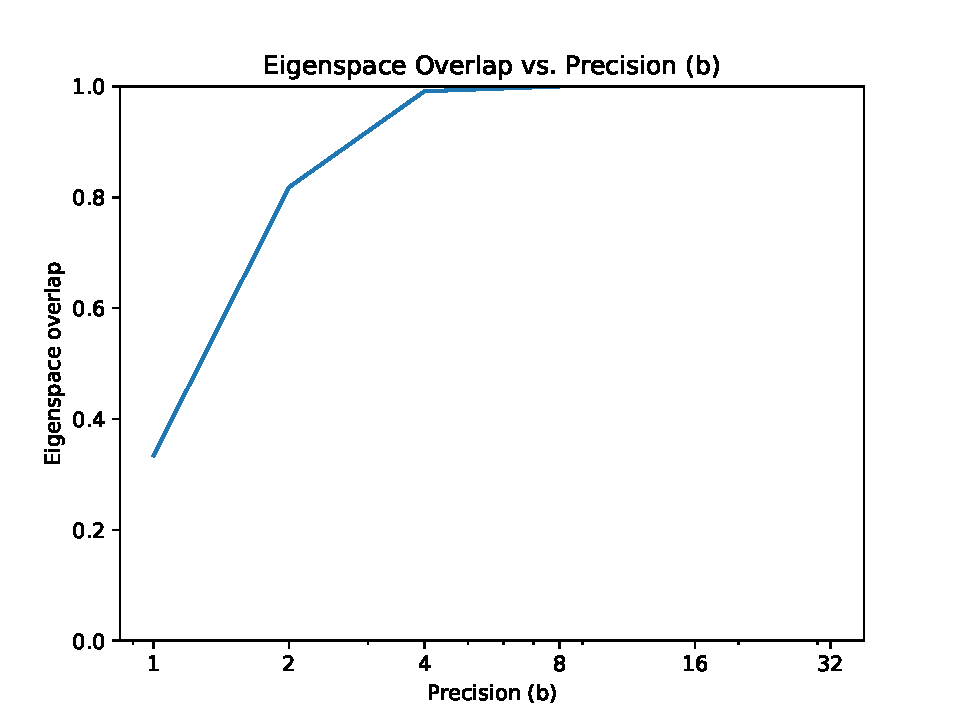
\includegraphics[width=\linewidth]{figures/micro_eig_overlap_vs_precision.pdf} 
%\end{tabular}
%\caption{Empirical Validation of Theorem~\ref{thm1}. We measure the eigenspace overlap of uniformly quantized embeddings with the uncompressed embedding for various precisions ($b\in\{1,2,4,8,16,32\}$), and observe the eigenspace overlap grows quickly as the precision grows.  For the uncompressed embedding, we generate a random matrix $X \in \RR^{10^5 \times 300}$, with each entry drawn uniformly at random in $[-\frac{1}{\sqrt{300}}, \frac{1}{\sqrt{300}}]$.}
%\label{fig:micro_eigoverlap_vs_prec}
%\end{figure}

\begin{figure*}
	\begin{tabular}{c c c c}
		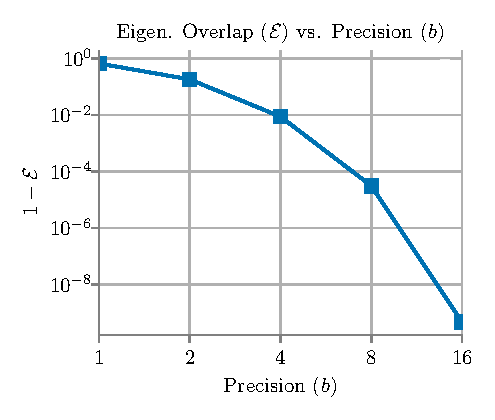
\includegraphics[width=0.23\linewidth]{figures/micro_eig_overlap_vs_prec.pdf} &
		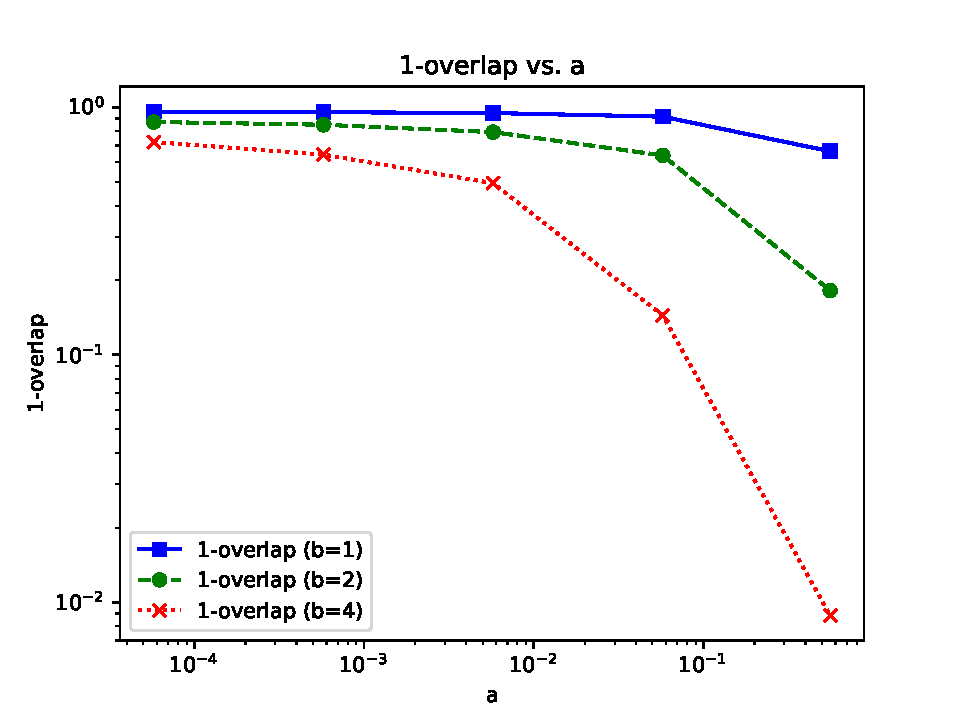
\includegraphics[width=0.23\linewidth]{figures/micro_eig_overlap_vs_a_multiple_prec_decay.pdf} &
		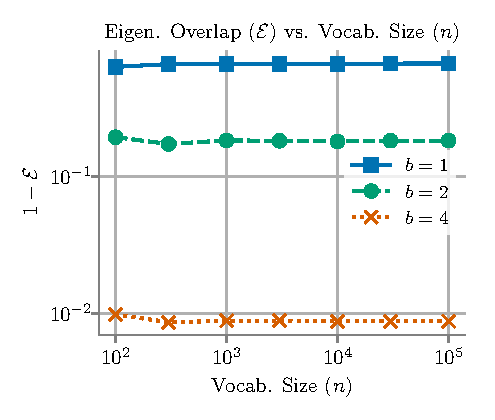
\includegraphics[width=0.23\linewidth]{figures/micro_eig_overlap_vs_n_vary_n.pdf} &
		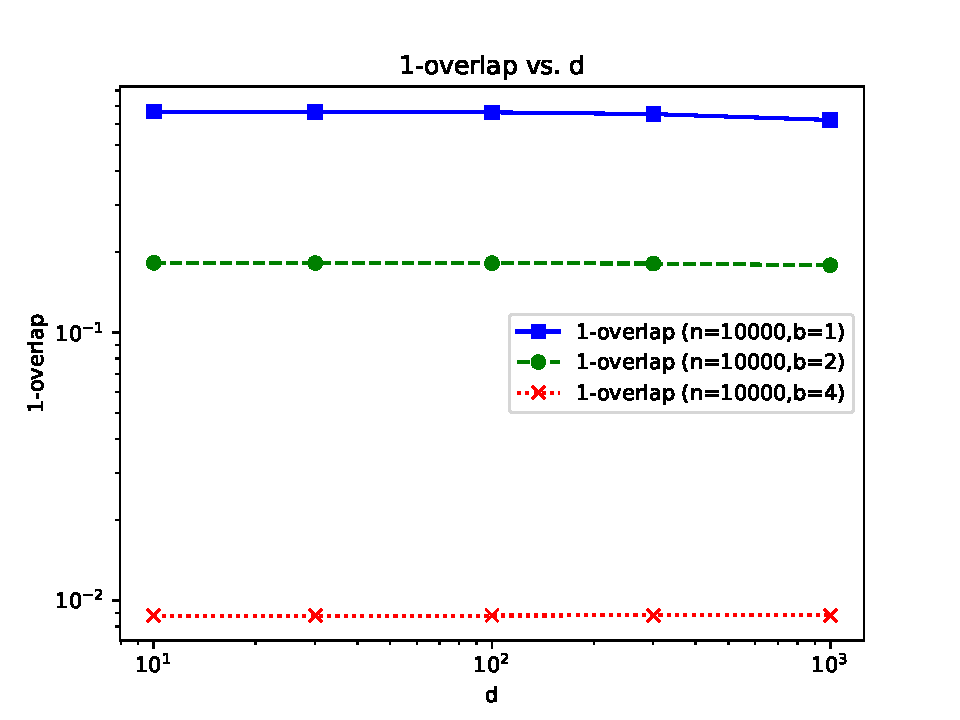
\includegraphics[width=0.23\linewidth]{figures/micro_eig_overlap_vs_d_vary_d.pdf} \\
		(a) & (b) & (c) & (d)
	\end{tabular}
	\caption{Empirical Validation of Theorem~\ref{thm1}. We measure the eigenspace overlap $\eigover$ of uniformly quantized embeddings with the uncompressed embedding for various precisions, values of $a$, vocabulary sizes $n$, and dimensions $d$.  We observe that $1-\eigover$ decays as the precision $b$ and scalar $a$ grow, and that $1-\eigover$ is largely unaffected by the vocabulary size $n$ and embedding dimension $d$.
	For more details on these experiments, see Section~\ref{sec:quant_embed}.}
	\label{fig:micro_eigoverlap}
\end{figure*}

%\subsection{Theory validation}
%	\begin{itemize}
%		\item Impact of quantization on overlap 
%			\begin{itemize}
% 				\item Exp 1: overlap vs precision for different dimensionality. Expectation: overlap increases with higher precision.
%				\item Exp2: overlap vs dimensionality for different precision. Expectation: overlap increases with dimensionality. This explains that under fix memory budget, using lower bits quantization can be beneficial
%			\end{itemize}
%		\item The impact of clipping on eigen-subspace overlap
%			\begin{itemize}
%				\item Simulation based experiments on subspace overlap as a function of different clipping threshold and precision. 
%				\item The way we introduce this in: in our main theorem, we assume the dynamic range is $O(1/\sqrt{d})$ as a consequence of the automatic clipping. We want to show here this is the case in practice and then discuss the specific way clipping influence eigenspace overlap.
%			\end{itemize}
%		\item Loop-back discussion on the large scale empirical experiments in Section~\ref{subsec:hard_explain}
%	\end{itemize}


%\paragraph{The impact of clipping on eigenspace overlap} 
%\begin{figure*}
%\begin{tabular}{c c c}
%	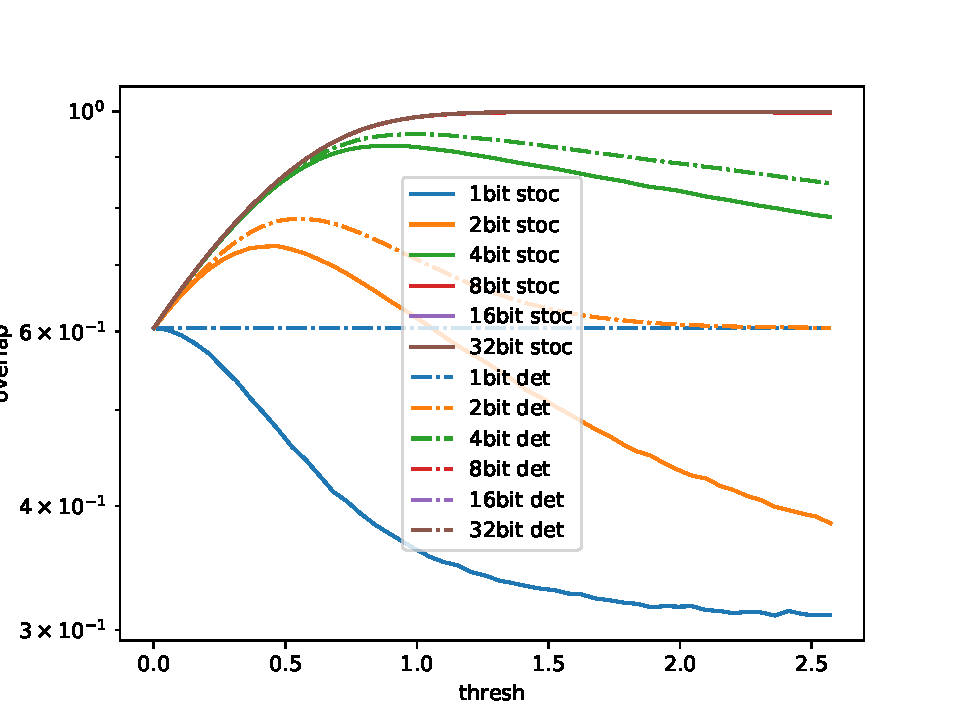
\includegraphics[width=0.3\linewidth]{figures/micro_overlap_and_clipping.pdf} &
%	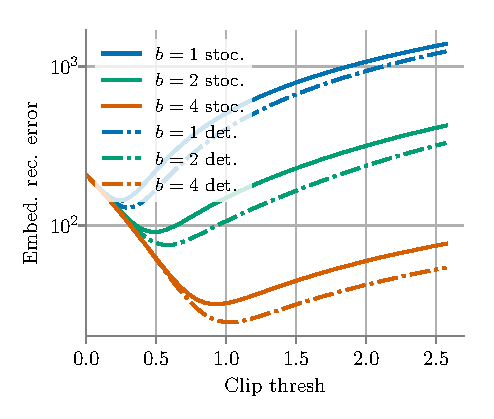
\includegraphics[width=0.3\linewidth]{figures/micro_rec_loss_and_clipping.pdf} &
%	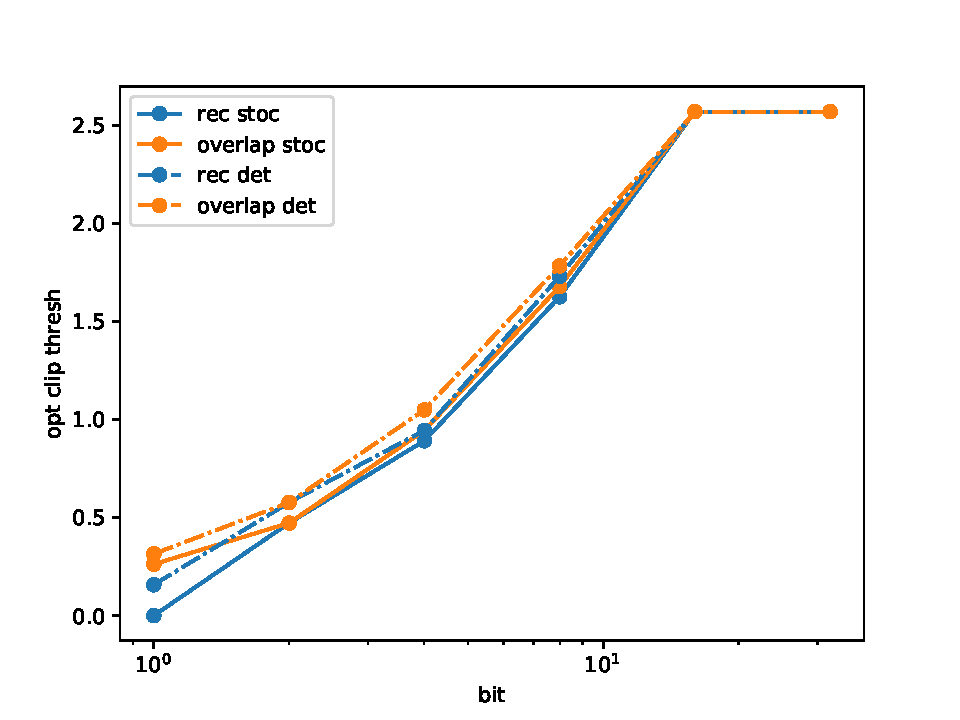
\includegraphics[width=0.3\linewidth]{figures/optimal_clip_thresh_and_bits.pdf} 
%\end{tabular}
%\label{fig:clipping_effect}
%\caption{Left: clipping thresh and overlap. Middle: clipping thresh and embedding reconstruction error. Right: optimal clipping threshold from overlap and embedding reconstruction error.}	
%\end{figure*}
\paragraph{The impact of clipping on eigenspace overlap} 
\begin{figure}
\begin{tabular}{c c c}
	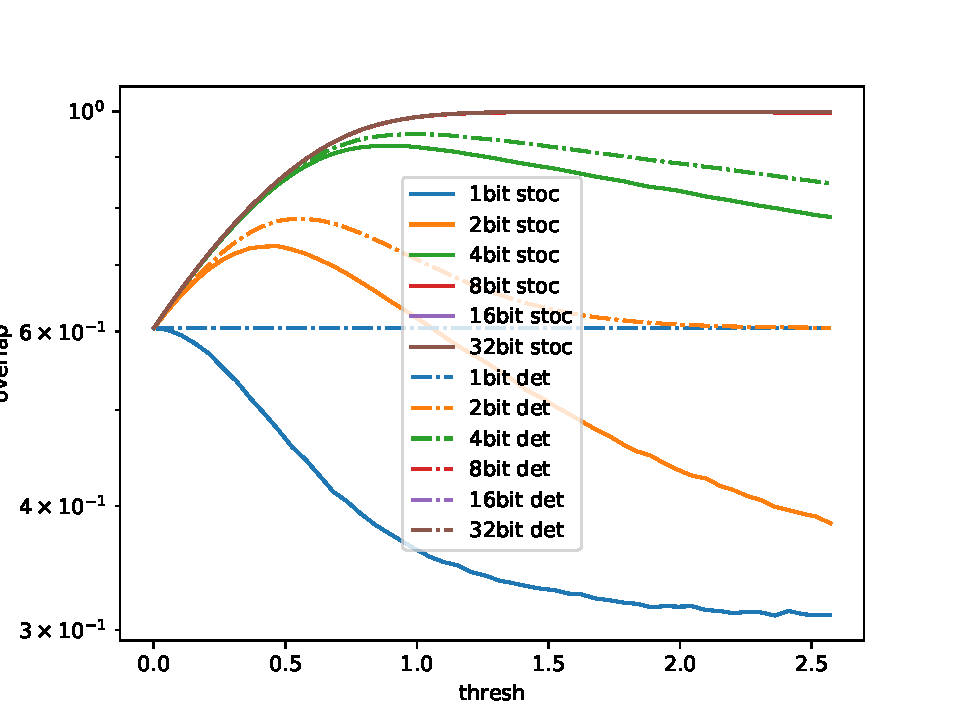
\includegraphics[width=0.45\linewidth]{figures/micro_overlap_and_clipping.pdf} &
	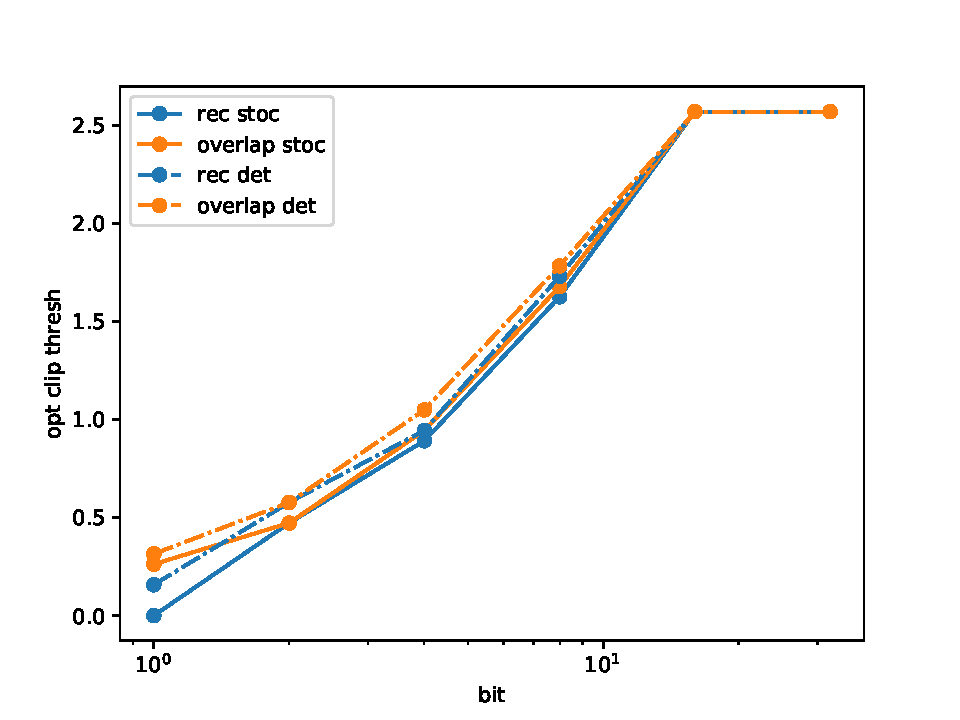
\includegraphics[width=0.45\linewidth]{figures/optimal_clip_thresh_and_bits.pdf}  \\
	(a) & (b)
\end{tabular}
\label{fig:clipping_effect}
\caption{\textbf{The impact of quantization on eigenspace overlap.} (a) The optimal eigenspace overlap for is often attained by aggressive clipping for low precision quantization, such as 1, 2 or 4-bits quantization. (b) Though the uniform quantization method search clipping threshold by minimizing embedding reconstruction, it produces consistent optimal clipping threshold with the value minimizing eigenspace overlap directly.}	
\end{figure}

As shown in Algorithm~\ref{alg:smallfry}, clipping is the first procedure in the uniform quantization method. It eliminates extremal entries in embedding, and can reduce quantization error level for the majority of entries with limited number of bits. To expose a more complete understanding of the generalization performance for the uniform quantization method, we demonstrate the impact of clipping to the downstream task performance. We show clipping is important because it can improve the eigenspace overlap, comparing to uniform quantization without clipping. In Figure~\ref{fig:clipping_effect} (a), we demonstrate the eigenspace overlaps attained with various clipping values for different number of bits for deterministic and deterministic quantization. In particular, we collect eigenspace overlap using the 300-dimensional GloVe pre-trained embedding trained on Wiki'14 corpus. We can observe that aggressive clipping is required to attain the optimal eigenspace overlap for low precision quantization with 1, 2 or 4 bits. For these quantization precision, the optimal eigenspace overlap can be larger using deterministic rounding than stochastic rounding; this can explain our empirical observation that deterministic rounding demonstrates better downstream task performance when using low quantization precision \todo{we need a pointer to somewhere maybe appendix?}. In Algorithm~\ref{alg:smallfry}, we search optimal clipping threshold by minimizing embedding reconstruction error instead of eigenspace overlap for better computational efficiency. Nonetheless, in Figure~\ref{fig:clipping_effect} (b), we can achieve similar optimal clipping threshold by minimizing eigenspace overlap directly across different quantization precision. 



